% Dokumentenart. Ersetze 12pt, falls die Schriftgröße anzupassen ist.
\documentclass[12pt]{scrartcl}

% Einbinden der Pakete, des Headers und der Formatierung.
% LaTeX Template für Abgaben an der Universität Stuttgart
% Autor: Sandro Speth
% Bei Fragen: Sandro.Speth@studi.informatik.uni-stuttgart.de
%-----------------------------------------------------------
% Modul fuer verwendete Pakete.
% Neue Pakete einfach einfuegen mit dem \usepackage Befehl:
% \usepackage[options]{packagename}
\usepackage[utf8]{inputenc}
\usepackage[T1]{fontenc}
\usepackage[ngerman]{babel}
\usepackage{lmodern}
\usepackage{graphicx}
\usepackage{float}
\usepackage[pdftex,hyperref,dvipsnames]{xcolor}
\usepackage{listings}
\usepackage[a4paper,lmargin={2cm},rmargin={2cm},tmargin={3.5cm},bmargin = {2.5cm},headheight = {4cm}]{geometry}
\usepackage{amsmath,amssymb,amstext,amsthm}
\usepackage[lined,algonl,boxed]{algorithm2e}
\usepackage{algorithmic}
\usepackage{multirow}
% alternative zu algorithm2e:
%\usepackage[]{algorithm} %counter mit chapter
%\usepackage{algpseudocode}
\usepackage{tikz}
\usepackage{hyperref}
\usepackage{url}
\usepackage[inline]{enumitem} % Ermöglicht ändern der enum Item Zahlen
\usepackage[headsepline]{scrlayer-scrpage} 
\usepackage{csquotes}
\pagestyle{scrheadings} 
\usetikzlibrary{automata,positioning,shapes.geometric,trees}

% LaTeX Template für Abgaben an der Universität Stuttgart
% Autor: Sandro Speth
% Bei Fragen: Sandro.Speth@studi.informatik.uni-stuttgart.de
%-----------------------------------------------------------
% Modul beinhaltet Befehl fuer Aufgabennummerierung,
% sowie die Header Informationen.

% Überschreibt enumerate Befehl, sodass 1. Ebene Items mit
\renewcommand{\theenumi}{(\alph{enumi})}
\renewcommand{\theenumii}{(\roman{enumii})}
% (a), (b), etc. nummeriert werden.
\renewcommand{\labelenumi}{\text{\theenumi}}
\renewcommand{\labelenumii}{\text{\theenumii}}

% Counter für das Blatt und die Aufgabennummer.
% Ersetze die Nummer des Übungsblattes und die Nummer der Aufgabe
% den Anforderungen entsprechend.
% Gesetz werden die counter in der hauptdatei, damit siese hier nicht jedes mal verändert werden muss
% Beachte:
% \setcounter{countername}{number}: Legt den Wert des Counters fest
% \stepcounter{countername}: Erhöht den Wert des Counters um 1.
\newcounter{sheetnr}
\newcounter{exnum}

% Befehl für die Aufgabentitel
\newcommand{\exercise}[1]{\section*{Exercise \theexnum\stepcounter{exnum}: #1}} % Befehl für Aufgabentitel

% Formatierung der Kopfzeile
% \ohead: Setzt rechten Teil der Kopfzeile mit
% Namen und Matrikelnummern aller Bearbeiter
\ohead{Hui Zeng}
% \chead{} kann mittleren Kopfzeilen Teil sezten
% \ihead: Setzt linken Teil der Kopfzeile mit
% Modulnamen, Semester und Übungsblattnummer
\ihead{Cloud Computing\\
Summer semester 2021\\
Lecture Notes Summary}

\definecolor{comments}{rgb}{0.41,0.54,0.21}
\definecolor{code}{rgb}{0,0,0}
\definecolor{keyword}{rgb}{0.77,0.48,0.57}
\definecolor{number}{rgb}{0.153,0.5,0}
\definecolor{codeBack}{rgb}{0.85,0.85,0.85}
\definecolor{string}{rgb}{0.81,0.57,0.47}

\lstdefinestyle{stdCode}{
	backgroundcolor=\color{codeBack},   
	commentstyle=\color{comments},
	literate=*{0}{{\textcolor{number}{0}}}{1}%
         {1}{{\textcolor{number}{1}}}{1}%
         {2}{{\textcolor{number}{2}}}{1}%
         {3}{{\textcolor{number}{3}}}{1}%
         {4}{{\textcolor{number}{4}}}{1}%
         {5}{{\textcolor{number}{5}}}{1}%
         {6}{{\textcolor{number}{6}}}{1}%
         {7}{{\textcolor{number}{7}}}{1}%
         {8}{{\textcolor{number}{8}}}{1}%
         {9}{{\textcolor{number}{9}}}{1}%
         {.0}{{\textcolor{number}{.0}}}{1}% Following is to ensure that only periods
         {.1}{{\textcolor{number}{.1}}}{1}% followed by a digit are changed.
         {.2}{{\textcolor{number}{.2}}}{1}%
         {.3}{{\textcolor{number}{.3}}}{1}%
         {.4}{{\textcolor{number}{.4}}}{1}%
         {.5}{{\textcolor{number}{.5}}}{1}%
         {.6}{{\textcolor{number}{.6}}}{1}%
         {.7}{{\textcolor{number}{.7}}}{1}%
         {.8}{{\textcolor{number}{.8}}}{1}%
         {.9}{{\textcolor{number}{.9}}}{1}%
         {\ }{{ }}{1}% handle the space
         ,%
	keywordstyle=\color{keyword},
	numberstyle=\tiny\color{number},
	stringstyle=\color{string},
	basicstyle=\ttfamily\scriptsize,
	breakatwhitespace=false,         
	breaklines=true,                 
	captionpos=b,                    
	keepspaces=true,                 
	numbers=left,                    
	numbersep=5pt,                  
	showspaces=false,                
	showstringspaces=false,
	showtabs=false,                  
	tabsize=2
}

\lstset{
	style=stdCode, language=Java,
  	literate={ö}{{\"o}}1
           {ä}{{\"a}}1
           {ü}{{\"u}}1
}

\tikzset{triangle/.style = {regular polygon, regular polygon sides=3 },
node rotated/.style = {rotate=180},
border rotated/.style = {shape border rotate=180},
astTerminal/.style = {regular polygon, regular polygon sides=3, inner sep=2.5pt, shape border rotate=180},
astLabel/.style = {right=3pt,font=\footnotesize\itshape},
astValue/.style = {below=5pt},
astLine/.style = {edge from parent fork down}
}
\graphicspath{{bilder/}}


% Counter für das Blatt und die Aufgabennummer.
\setcounter{sheetnr}{0} % Nummer des Übungsblattes
\setcounter{exnum}{1} % Nummer der Aufgabe

\newcommand*\circled[1]{\tikz[baseline=(char.base)]{
		\node[shape=circle,draw,inner sep=2pt] (char) {#1};}}     % number in circles
% Beginn des eigentlichen Dokuments
\begin{document}
	\pagenumbering{roman}
	\title{Business Analytics}
\author{Hui Zeng \thanks{All notes are summarized from the lecture and tutorial materials provided by Prof. Martin Bichler and his DSS team. Images are retrieved from the lecture as well as tutorial slides.}}
\date{Winter Semester 2020-2021}
\maketitle

\newpage
	\newpage
	\setcounter{tocdepth}{2}
	
	\tableofcontents
	\newpage
	\flushleft
	
	\pagenumbering{arabic}
	\section{Introduction}
Different IT-trends boosts the need for cloud computing:
\begin{itemize}
	\item Outsourcing, either infrastructure or management
	\item IT as a service: pay per use
	\item Re-centralization of data: similar to data centers, cloud be provided as a central place for data storage.
	\item Resource sharing instead of over-provisioning: same resource can be used for multiple purposes
	\item Server consolidation: instead of having multiple physical servers, with each dedicated to a certain service, servers are virtualized and put on one/reduced number of physical machines.     
	\item Scalable computing
	\item Application dynamism: amount of request on web changes over time.
	\item Green computing, big data, stream processing, IoT, machine learning, etc.
\end{itemize}

\paragraph{Cloud Computing} the definition is mainly divided by
\begin{itemize}
	\item ubiquitous, convenient, on-demand network access to a \textbf{shared pool of configurable computing resources} (eg: networks, servers, storage, applications, services)
	\item resources can be \textbf{rapidly provisioned} and released with \textbf{minimal management effort} or service provider interaction
	\item cloud model is composed of 
	\begin{itemize}		
		\item 3 service models
		\item 4 deployment models
		\item 5 essential characteristics
	\end{itemize}
\end{itemize}

\subsection{3 Service Models: IaaS, PaaS and SaaS}
Three service models, ranking from outsourcing the least to the most: IaaS $\rightarrow$ PaaS $\rightarrow$ SaaS.

\subsubsection{IaaS: Infrastructure as a Service}
\begin{itemize}
	\item Offering: provision processing, storage, networks, other fundamental computing resources
	\item Rights as consumer: 
	\begin{itemize}
		\item deploy and run \textbf{arbitrary} software, including \textbf{operating systems and applications}
		\item control over OS, storage, deployed applications
		\item limited control of select networking components
	\end{itemize}
	\item No control as consumer:
	\begin{itemize}
		\item underlying cloud infrastructure
	\end{itemize}
	
	
\end{itemize}
\subsubsection{PaaS: Platform as a Service}
\begin{itemize}
	\item Offering: application infrastructure services(eg: development platforms, libraries, tools, databases) through client interface
	\item Rights as consumer:
	\begin{itemize}
		\item limited user-specific application configuration settings
	\end{itemize}
	\item No control as consumer:
	\begin{itemize}
		\item underlying cloud infrastructure
		\item network, servers, storage, OS
		\item individual application capabilities
	\end{itemize}
	\item Example: MS Azure, Amazon FaaS, Google application engine
\end{itemize}
\subsubsection{SaaS: Software as a Service}
\begin{itemize}
	\item Offering: provider's applications on cloud through client interface
	\item Rights as consumer:
	\begin{itemize}
		\item limited user-specific application configuration settings
	\end{itemize}
	\item No control as consumer:
	\begin{itemize}
		\item underlying cloud infrastructure
		\item network, servers, OS, storage
		\item individual application capabilities
	\end{itemize}
\end{itemize}
\begin{figure}[H]
	\centering
	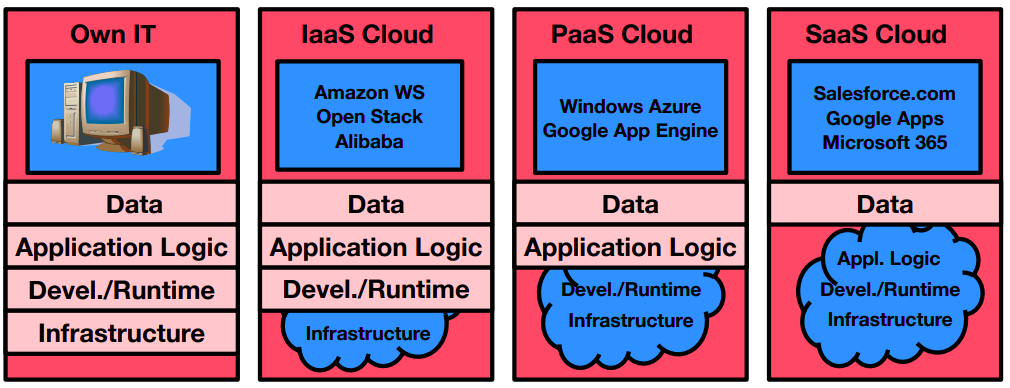
\includegraphics[width=\textwidth]{servicemodels.png}
	%\caption{Comparison over the service models}
\end{figure}
\begin{figure}[H]
	\centering
	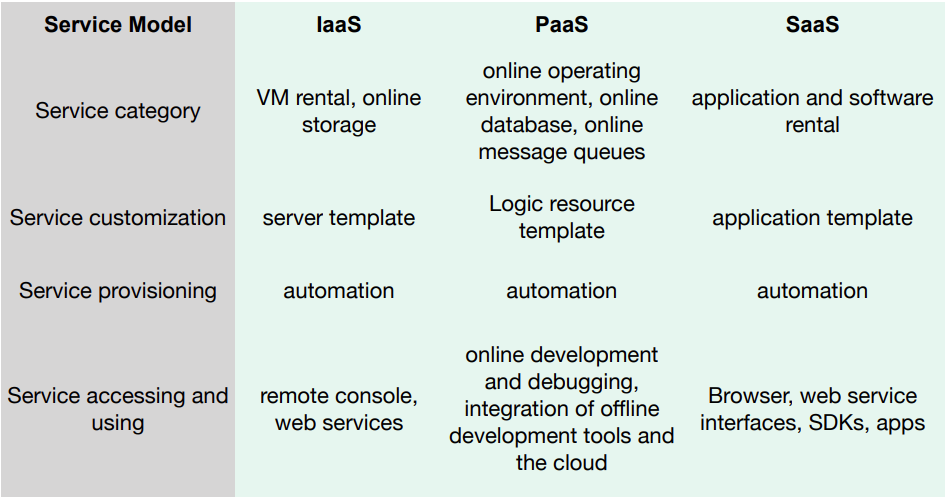
\includegraphics[width=0.8\textwidth]{servicemodel1.png}
	%\caption{Comparison over the service models}
\end{figure}\begin{figure}[H]
\centering
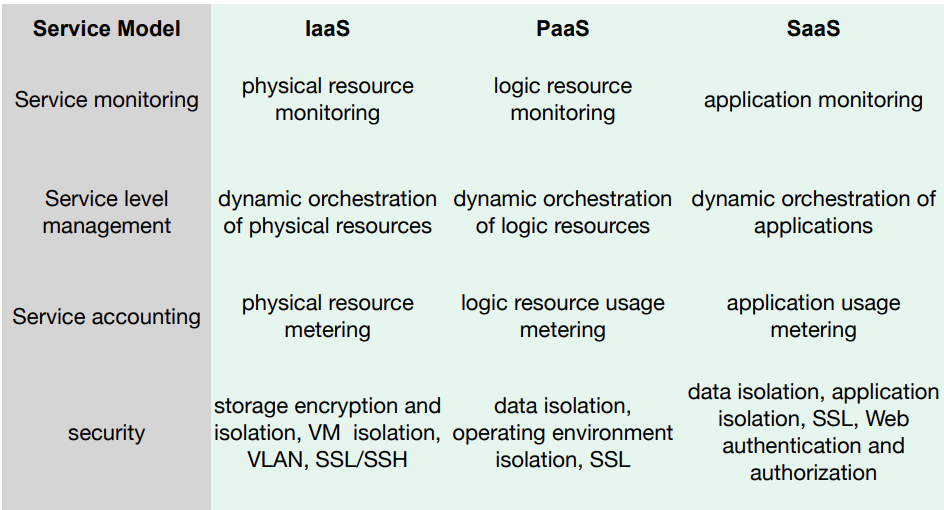
\includegraphics[width=0.8\textwidth]{servicemodel2.png}
%\caption{Comparison over the service models}
\end{figure}
\subsection{4 Deployment Models: Private, Community, Public, Hybrid}
\begin{itemize}
	\item Private Cloud:
	\begin{itemize}
		\item service offered \textbf{via private network} for \textbf{single client}.
	\end{itemize}
	\item Community Cloud:
	\begin{itemize}
		\item service offered to \textbf{a specific group of clients}.
	\end{itemize}
	\item Public Cloud:
	\begin{itemize}
		\item service offered \textbf{over Internet via Web-application} or third-party provider for \textbf{everyone}.
	\end{itemize}
	\item Hybrid Cloud: combination of public and private cloud.
\end{itemize}

\subsection{5 Essential Characteristics}
\begin{itemize}
	\item \textbf{on-demand self-service}: 
	\begin{itemize}
		\item able to \textbf{provision computing capabilities} unilaterally(no interaction required with provider).
	\end{itemize}
	
	\item \textbf{broad network access}: 
	\begin{itemize}
		\item capabilities can be available and accessed through by \textbf{diversely thin or thick client platforms} (mobile, tablets, cable, etc.)
	\end{itemize}
	
	\item \textbf{resource pooling}: 
	\begin{itemize}
		\item \textbf{multi-tenant model} is used, multiple customers shares the computing capabilities at the same time, according to their self-customized demand. Specification of resource location can be possible at higher abstraction level.
	\end{itemize}
	 
	\item \textbf{rapid elasticity}: 
	\begin{itemize}
		\item computing capabilities can be \textbf{elastically provisioned and released} in any quantity at any time. The process can be automated or scaled according to dynamic demand.
	\end{itemize}
	\item \textbf{measured service}: 
	\begin{itemize}
		\item automatically control and optimize resource use by \textbf{leveraging a metering capability}. Resource usage can be monitored, controlled and reported.
	\end{itemize}
\end{itemize}


\subsection{Pros \& Cons of Clouds}
\begin{itemize}
	\item Advantages:

\begin{itemize}
	\item scalability, elasticity
	\item rapid deployment
	\item no capital investment for physical resources
	\item outsourcing of infrastructure management
	\item limited access to on-premise servers
	\item fault tolerance: multiple servers have data replicas, if one node fails, other nodes will replace.
	\item collaboration
\end{itemize}
	\item Disadvantages:
	\begin{itemize}
		\item no control over security, based on ''trust''.
		\item no control over hardware/infrastructure
		\item vendor lockin: service is not standardized, not compatible to other vendors.
		\item cost on monthly fees: if demand for same computational power is constant, fee may be higher than building own hardware. Only recommendable for dynamic demand.
		\item breaking SLAs: your performance may be influenced by other tenants(multi-tenant model).
	\end{itemize}
\end{itemize}

\end{document}
